%  The AAU Poster Theme.
%  2013-05-08 v. 1.1.0
%  Copyright 2013 by Jesper Kjær Nielsen <jkn@es.aau.dk>
%
%  This is free software: you can redistribute it and/or modify
%  it under the terms of the GNU General Public License as published by
%  the Free Software Foundation, either version 3 of the License, or
%  (at your option) any later version.
%
%  This is distributed in the hope that it will be useful,
%  but WITHOUT ANY WARRANTY; without even the implied warranty of
%  MERCHANTABILITY or FITNESS FOR A PARTICULAR PURPOSE.  See the
%  GNU General Public License for more details.
%
%  You can find the GNU General Public License at <http://www.gnu.org/licenses/>.
\documentclass[a0paper,portrait]{baposter}
\usepackage{xspace}
\usepackage{xcolor}
\usepackage{xcolor}
\usepackage[utf8]{inputenc}
\usepackage[english]{babel}
% \usepackage{helvet}
% \usepackage{lmodern}
\renewcommand{\familydefault}{\sfdefault}
\usepackage[T1]{fontenc}
\usepackage{lipsum}
\usepackage{tabularx}
\usepackage[misc]{ifsym}
\usepackage{fixltx2e}
\usepackage{gensymb}
\usepackage{listings}
\usepackage{tcolorbox}
\usepackage{relsize}

\usepackage{caption}
\captionsetup{
  font=small,% set font size to footnotesize
  labelfont=bf % bold label (e.g., Figure 3.2) font
}

% Make the standard latex tables look so much better
\usepackage{array,booktabs}

% For creating beautiful plots
\usepackage{tikz}
\usetikzlibrary{positioning}
\usetikzlibrary{shapes,arrows,backgrounds,fit,shapes.geometric,calc}
\usetikzlibrary{pgfplots.groupplots}
\usetikzlibrary{patterns}
\usepackage{pgfplots}
\usepackage{pgfplotstable}

\usepackage{amsmath}
\usepackage{amssymb}

\usepackage{microtype}

% http://en.wikibooks.org/wiki/LaTeX/Colors
\selectcolormodel{RGB}
% define the three aau colors
\definecolor{posterbg}{RGB}{230,230,255}% background colour for the poster

%%%%%%%%%%%%%%%%%%%%%%%%%%%%%%%%%%%%%%%%%%%%%%%%
% Lists
% http://en.wikibooks.org/wiki/LaTeX/List_Structures
%%%%%%%%%%%%%%%%%%%%%%%%%%%%%%%%%%%%%%%%%%%%%%%%
% Easier configuration of lists
\usepackage{enumitem}
\usepackage{ragged2e}
%configure itemize
\setlist{%
  topsep=3pt,% set space before and after list
  noitemsep,% remove space between items
  itemsep=1pt,% and add a tiny bit back in
  labelindent=\parindent,% set the label indentation to the paragraph indentation
  leftmargin=*,% remove the left margin
  font=\color{black}\normalfont, %set the colour of all bullets, numbers and descriptions to aaublue1
  after=\RaggedRight, % make list ragged
}
\setdescription{font=\color{blue!50!black}\normalfont\bfseries}

%%%%%%%%%%%%%%%%%%%%%%%%%%%%%%%%%%%%%%%%%%%%%%%%
% Misc
%%%%%%%%%%%%%%%%%%%%%%%%%%%%%%%%%%%%%%%%%%%%%%%%
% change/remove some names
\addto{\captionsenglish}{
  %remove the title of the bibliograhpy
  \renewcommand{\refname}{\vspace{-0.7em}}
  %change Figure to Fig. in figure captions
  \renewcommand{\figurename}{Fig.}
}
% create links
\usepackage{url}
% note that the hyperref package is currently incompatible with the baposter class

%\makeatletter
%\newcommand\notsotiny{\@setfontsize\notsotiny\@vipt\@viipt}
%\makeatother
\newcommand{\lstfont}[1]{\color{#1}\bfseries\scriptsize\ttfamily}

% Change the empty line interline spacing for listings
\makeatletter 
\lst@AddToHook{OnEmptyLine}{\vspace{\dimexpr-\baselineskip+0.8\smallskipamount}}
\makeatother

\lstdefinestyle{PosterPython}{
  showstringspaces=false,
  frame=single,
  % backgroundcolor=\color{white},
  basicstyle=\lstfont{black},
  identifierstyle=\lstfont{blue!30!black},
  keywordstyle=\lstfont{red!50!magenta},
  numberstyle=\lstfont{white},
  stringstyle=\lstfont{blue!70!black},
  commentstyle=\lstfont{green!10!black},
  language=python,
  morekeywords={as},
}

\lstdefinestyle{PosterOutput}{
  showstringspaces=false,
  frame=single,
  backgroundcolor=\color{white!95!black},
  basicstyle=\lstfont{black}
}


%%%%%%%%%%%%%%%%%%%%%%%%%%%%%%%%%%%%%%%%%%%%%%%%
% Macros
%%%%%%%%%%%%%%%%%%%%%%%%%%%%%%%%%%%%%%%%%%%%%%%%
\colorlet{emph}{blue}
\newcommand{\todo}[1]{{\color{red}#1}}
\newcommand{\hilight}[1]{{\color{blue}\textbf #1}}
\newcommand{\arborname}{Arbor\xspace}
\newcommand{\arbor}{{\textcolor{blue!30!black}{\arborname}}\xspace}
\newcommand{\arboremph}{{\textcolor{emph!70!black}{\arborname}}\xspace}
\newcommand{\julich}{FZ-J\"ulich\xspace}
\newcommand{\tb}[1]{\textbf{\textcolor{blue!50!red}{#1}}\xspace}
\newcommand{\centerheader}[1]{\begin{center}\bfseries\Large{#1}\end{center} \vspace{-6pt}}
\newcommand{\imageheader}[1]{\begin{center}\bfseries\large{#1}\end{center} \vspace{-2pt}}

\newcommand\neuron{{\relsize{-2}NEURON}\xspace}
\newcommand\nest{{\relsize{-2}NEST}\xspace}
\newcommand\tvb{{\relsize{-2}TVB}\xspace}

\newcommand{\newemph}[1]{{\color{emph}#1}}

\pgfplotsset{every tick label/.append style={font=\footnotesize}}

%%%%%%%%%%%%%%%%%%%%%%%%%%%%%%%%%%%%%%%%%%%%%%%%
% Document Start 
%%%%%%%%%%%%%%%%%%%%%%%%%%%%%%%%%%%%%%%%%%%%%%%%
\begin{document}
%%%%%%%%%%%%%%%%%%%%%%%%%%%%%%%%%%%%%%%%%%%%%%%%
% Some changes that cannot be made in the preamble
%%%%%%%%%%%%%%%%%%%%%%%%%%%%%%%%%%%%%%%%%%%%%%%%
% set the background of the poster
\background{
  \begin{tikzpicture}[remember picture,overlay]%
    %the poster background color
    \fill[fill=white] (current page.north west) rectangle (current page.south east);

    %the header
    \fill [fill=white] (current page.north west) rectangle ([yshift=-\headerheight] current page.north east);
  \end{tikzpicture}
}
% if you want to reduce the space before and after equations, use and adjust
% the following lines
%\addtolength{\abovedisplayskip}{-2mm}
%\addtolength{\belowdisplayskip}{-2mm}

%%%%%%%%%%%%%%%%%%%%%%%%%%%%%%%%%%%%%%%%%%%%%%%%
% General poster setup
%%%%%%%%%%%%%%%%%%%%%%%%%%%%%%%%%%%%%%%%%%%%%%%%
\begin{poster}{
    %general options for the poster
    grid=false,
    columns=3,
    % these two control space between and padding inside
    % the poster boxes
    colspacing=3mm,
    boxpadding=2mm,
    %
    headerheight=0.1\textheight,
    background=user,
    headerborder=closed,
    borderColor=blue!40!black,
    headershape=rectangle,
    headershade=plain,
    headerColorOne=blue!15,
    textborder=rectangle,
    boxshade=plain,
    boxColorOne=white,
    headerFontColor=black,
    headerfont=\Large\sf,
    linewidth=1pt
}

%the Eye Catcher (the logo on the left)
{
  \begin{tikzpicture}[remember picture, overlay]
    \node [anchor=north west,xshift=0.02\paperwidth,yshift=-0.03\headerheight] at (current page.north west) {
      \includegraphics[height=0.4\headerheight]{HBP_logo.jpg}
    };
    \node [anchor=north west,xshift=0.32\paperwidth,yshift=-0.10\headerheight] at (current page.north west) {
      \includegraphics[height=0.25\headerheight]{julich_logo.pdf}
    };
    \node [anchor=north west,xshift=0.59\paperwidth,yshift=-0.10\headerheight] at (current page.north west) {
      \includegraphics[height=0.25\headerheight]{cscs_logo.pdf}
    };
    \node[anchor=north west,xshift=0.8\paperwidth,yshift=-0.05\headerheight] at (current page.north west) {
      \includegraphics[height=0.4\headerheight]{images/eu_logo.png}
    };
  \end{tikzpicture}
  \vspace{0.3\headerheight}
}
%the poster title
{ \Huge
  \textbf{\arbor} \\[0.1\baselineskip]
\large 
  A morphologically detailed neural network simulation library for modern high performance computer architectures \\[0.2\baselineskip]
  \small
    Ben Cumming\textsuperscript{a}\!\!,~~Stuart Yates\textsuperscript{a}\!\!,~~Nora Abi Akar\textsuperscript{a}\!\!,~~Anne K\"usters\textsuperscript{b}\!\!,~~Wouter Klijn\textsuperscript{b}\!\!,~~Alexander Peyser\textsuperscript{b}\\
    \textsuperscript{a}Swiss National Supercomputing Center \hspace{2mm}\textsuperscript{b}Simulation Lab Neuroscience, Forschungszentrum \julich
}
%the author(s)
{\small
    \vspace{1em} Ben Cumming, \\[0.5em]
    Swiss National Supercomputing Center (CSCS), Switzerland\\
}

%%%%%%%%%%%%%%%%%%%%%%%%%%%%%%%%%%%%%%%%%%%%%%%%
% LEFT HAND SIDE OF POSTER
%%%%%%%%%%%%%%%%%%%%%%%%%%%%%%%%%%%%%%%%%%%%%%%%

%%%%%%%%%%%%%%%%%%%%%%%%%%%%%%%%%%%%%%%%%%%%%%%%
\begin{posterbox}[name=motivation,column=0,row=0,span=2]{What is \arbor?}
    \begin{center}\large
        \colorbox{yellow!20}{\arbor is a library for the simulation of large networks of morphologically-detailed}
        \\
        \colorbox{yellow!20}{neurons for all HPC systems in the HBP.}
        \\
        Runs on GPU systems, vectorized multicore, Intel KNL and laptops. \\
        Modular design for extensibility to new computer architectures.
    \end{center}

    \begin{center}
        \colorbox{yellow!20}{\large \arbor is developed by a team from HPC centers.}
        \\[2pt]
            \centering CSCS and \julich in SGA2 \newemph{WP 7.3}.
    \end{center}
\end{posterbox}
%%%%%%%%%%%%%%%%%%%%%%%%%%%%%%%%%%%%%%%%%%%%%%%%

%%%%%%%%%%%%%%%%%%%%%%%%%%%%%%%%%%%%%%%%%%%%%%%%
\begin{posterbox}[name=progress,column=0,below=motivation,span=1]{Progress \& Features}
    \raggedright
    \newemph{Features added since the last HBP Summit:}
    \vspace{7pt}
    \begin{itemize}
        \item Vectorization of NMODL kernels with vector intrinsics. See \emph{Vectorization} box below.
        \item A spike communication and event system that scales with negligible overheads to very large models and clusters.
        \item A new task-based threading implementation.
        \item CMake installable target and simple configuration for users of the \arbor library.
        \item Fine-grained allocation of CPU and GPU resources.
        \item An API for receiving spikes from external simulators.
    \end{itemize}

    \vspace{7pt}
    \newemph{Features coming soon to \arboremph include:}
    \vspace{7pt}
    \begin{itemize}
        \item A Python wrapper. See the \emph{Python Interface} box for details.
        \item Gap junctions.
        \item Coupling with \nest \& \tvb.
        \item Coupling with in-situ visualization and analytics.
        \item A benchmark and validation suite.
        \item Higher-order time stepping and error control.
    \end{itemize}
    \vspace{-4pt}
    \begin{center}
    \colorbox{yellow!20}{
        \begin{minipage}{0.9\textwidth}
            \centering
            Talk to us about features that you need.
        \end{minipage}
    }
    \end{center}

    \vspace{0pt}
\end{posterbox}
%%%%%%%%%%%%%%%%%%%%%%%%%%%%%%%%%%%%%%%%%%%%%%%%

%%%%%%%%%%%%%%%%%%%%%%%%%%%%%%%%%%%%%%%%%%%%%%%%
\begin{posterbox}[name=vector,column=0,below=progress,span=1]{Vectorization}
    \arbor uses a new library for SIMD vectorization.

    \begin{itemize}
        \item Generic vectorized code is generated from NMODL ion channel and synapse descriptions.
        \item Adding support for new SIMD architectures is straightforward.
    \end{itemize}

    Speedup of \newemph{total time to solution} with vectorization is $0.5$--$2.5\times$.
    The plot below shows speedup on a range of Intel CPUs, both for single core and for a full socket.

    \vspace{-1pt}
    \imageheader{Vectorization Speedup of Wall Time}
    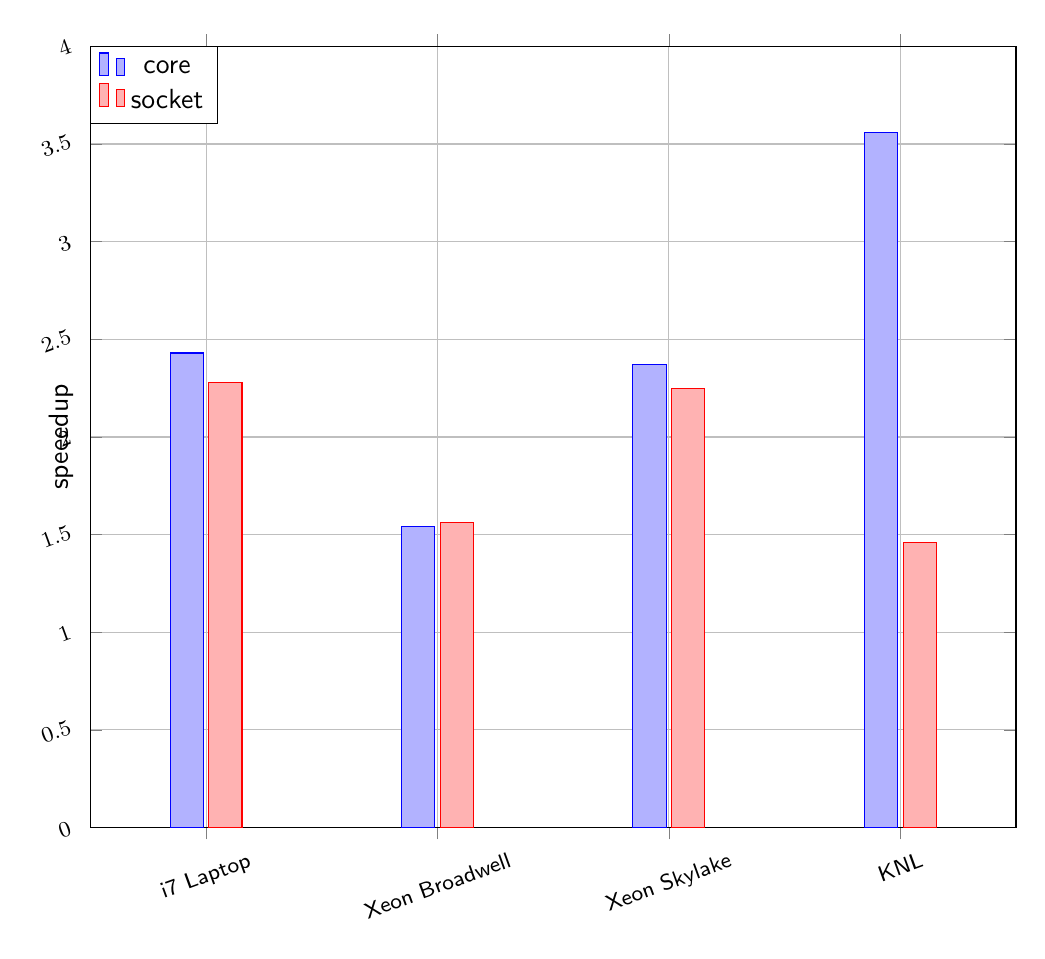
\begin{tikzpicture}
       \begin{axis}[ylabel=speeedup,
            ybar,
            width=1.1\textwidth,
            xmin=50, xmax=450,
            ymin=0, ymax=4,
            xtick={100,200,300,400},
            xticklabels={i7 Laptop, Xeon Broadwell, Xeon Skylake, KNL},
            ylabel style={yshift=-20pt},
            yticklabel style={xshift=-2pt},
            legend style = {at={(0,1)}, anchor=north west},
            grid=major,
            tick label style={rotate=20},
            bar width=12pt]
           % single core
           \addplot coordinates {
                    (100,2.43) (200,1.54) (300,2.37) (400,3.56)};
           % node/socket
           \addplot coordinates {
                    (100,2.28) (200,1.56) (300,2.25) (400,1.46)};

           \legend{core, socket}
       \end{axis}
    \end{tikzpicture}

    \vspace{-1pt}
\end{posterbox}
%%%%%%%%%%%%%%%%%%%%%%%%%%%%%%%%%%%%%%%%%%%%%%%%

%%%%%%%%%%%%%%%%%%%%%%%%%%%%%%%%%%%%%%%%%%%%%%%%
\begin{posterbox}[name=python,column=1,below=motivation,span=1]{Python Interface}
    A Python wrapper for \arbor will be released this year.
    \begin{itemize}
        \item Simple wrappper of the C++ API.
        \item Basis for PyNN integration.
        \item Working prototype with MPI \& GPU on Cray.
    \end{itemize}

    \vspace{-2pt}
    \begin{center}
    \colorbox{yellow!20}{
        \begin{minipage}{0.8\textwidth}
            \centering
        Ask us for a demonstration of the Python wrapper running in a Jupyter notebook on Piz Daint.
        \end{minipage}
    }
    \end{center}

    \vspace{2pt}

    Below is a simple example of defining, building and running a network with 4 soma-only cells:

    \vspace{2pt}

\lstinputlisting[style=PosterPython]{pyarb-example.py}

\vspace{0pt}

\begin{lstlisting}[style=PosterOutput]
cell 0 at    5.375 ms
cell 1 at   15.700 ms
cell 2 at   26.025 ms
cell 3 at   36.350 ms
cell 0 at   46.675 ms
cell 1 at   57.000 ms
cell 2 at   67.325 ms
cell 3 at   77.650 ms
cell 0 at   87.975 ms
cell 1 at   98.300 ms
\end{lstlisting}
\vspace{-4pt}

\end{posterbox}
%%%%%%%%%%%%%%%%%%%%%%%%%%%%%%%%%%%%%%%%%%%%%%%%


%%%%%%%%%%%%%%%%%%%%%%%%%%%%%%%%%%%%%%%%%%%%%%%%
% RIGHT HAND SIDE OF POSTER
%%%%%%%%%%%%%%%%%%%%%%%%%%%%%%%%%%%%%%%%%%%%%%%%

%%%%%%%%%%%%%%%%%%%%%%%%%%%%%%%%%%%%%%%%%%%%%%%%
\begin{posterbox}[name=plots,column=2,row=0,span=1]{Performance}
    {
        \tiny
        \colorbox[HTML]{FCF3CF}{%
            \begin{tabularx}{0.95\textwidth}{l|X}
          daint-mc  & Cray XC40: 2$\times$ 18-core Broadwell per node\smallskip\\
          daint-gpu & Cray XC50: 1$\times$P100 GPU per node\smallskip\\
              cells & 150 compartments \& 10,000 synapses per cell\\
                    & Passive dendrites, Hodgkin-Huxley soma\smallskip\\
            network & ring network\smallskip\\
           duration & 100\,ms\\
            \end{tabularx}
        }
    }
    \vskip4pt
    \imageheader{Single Node Scaling}
    \vspace{-5pt}
    { \small
        This benchmark scales a simple ring model on a single node of Piz Daint.
    }
    \vskip8pt
    \tikzset{>=stealth', pil/.style={ ->, color=black!60, thick, } }
\begin{tikzpicture}
    \begin{loglogaxis}[
        height=0.7\textwidth,
        width=\textwidth,
        xmin=64,xmax=16384,
        ymin=0.1, ymax=2000,
        xtick={64, 128, 256, 512, 1024, 2048, 4096, 8193, 16386},
        xticklabels={64, 128, 256, 512, 1k, 2k, 4k, 8k, 16k},
        ytick={1, 10, 60, 600, 1800},
        yticklabels={1s, 10s, 1m, 10m, 30m},
        %tick={0.1, 1, 10, 100, 1000},
        %yticklabels={0.1, 1, 10, 100, 1000},
        ylabel=wall time (s),
        xlabel=cells,
        xticklabel style={yshift=-2pt},
        yticklabel style={xshift=-2pt},
        legend style = {at={(1,0)}, anchor=south east},
        line width=1pt,
        every axis y label/.style=
            {at={(ticklabel cs:0.5)},rotate=90,anchor=near ticklabel},
        grid=major]

        \addplot[color=orange, mark=*, mark size=1.5, mark options={fill=white}]
            table[x=cells,y=nrnmc_wall] {./images/nrn_arb.tbl};
        \addplot[color=blue, mark=*, mark size=1.5, mark options={fill=white}]
            table[x=cells,y=arbmc_wall] {./images/nrn_arb.tbl};
        \addplot[color=red, mark=*, mark size=1.5, mark options={fill=white}]
            table[x=cells,y=arbgpu_wall] {./images/nrn_arb.tbl};

        \node[above, fill=orange!15, align=center, inner sep=1mm]
              (n1) at (axis cs:512,600){\tiny largest Neuron model fit in 64~GB};
        \path[pil,->] (n1.east) edge (axis cs:7000,1200);

       \legend{ {\scriptsize Neuron},
                {\scriptsize Arbor-mc},
                {\scriptsize Arbor-gpu},
              };
    \end{loglogaxis}
\end{tikzpicture}


    { \small
    \begin{itemize}
        \item \arbor's efficient multicore memory layout gives perfect scaling.
        \item \neuron scales poorly from 64--256 cells as cache utilization decreases.
    \end{itemize}
    }

    \vskip8pt

    %\imageheader{Speedup \arbor vs \neuron}
    This plot shows the \newemph{speedup of \arboremph relative to \neuron} for the single node test above.

    \vskip8pt
    \tikzset{>=stealth', pil/.style={ ->, color=black!60, thick, } }
\begin{tikzpicture}
    \begin{axis}[
        xmode=log,
        height=0.7\textwidth,
        width=\textwidth,
        xmin=64,xmax=8192,
        ymin=0, ymax=35,
        xtick={64, 128, 256, 512, 1024, 2048, 4096, 8193, 16386},
        xticklabels={64, 128, 256, 512, 1k, 2k, 4k, 8k, 16k},
        ytick={0,5,10,15,20,25,30,35},
        ylabel=speedup,
        xlabel=cells,
        xticklabel style={yshift=-2pt},
        yticklabel style={xshift=-2pt},
        legend style = {at={(1,0.2)}, anchor=south east},
        line width=1pt,
        every axis y label/.style=
            {at={(ticklabel cs:0.5)},rotate=90,anchor=near ticklabel},
        grid=major]

        %\addplot[color=orange, mark=*, mark size=1.5, mark options={fill=white}]
            %table[x=cells,y expr=1] {./images/nrn_arb.tbl};
        \addplot[color=blue, mark=*, mark size=1.5, mark options={fill=white}]
            table[x=cells,y expr=\thisrow{arbmc_rate}/\thisrow{nrnmc_rate}] {./images/nrn_arb.tbl};
        \addplot[color=red, mark=*, mark size=1.5, mark options={fill=white}]
            table[x=cells,y expr=\thisrow{arbgpu_rate}/\thisrow{nrnmc_rate}] {./images/nrn_arb.tbl};

       \legend{
                {\scriptsize Arbor-mc},
                {\scriptsize Arbor-gpu},
              };
    \end{axis}
\end{tikzpicture}


    { \small
        \begin{itemize}
        \item For few cells per core \neuron is 5--10$\times$ slower.
        \item With more than 7 cells per core \arbor is over $20\times$ faster.
        \item \arbor's GPU backend is efficient with 1000 or more cells per GPU.
        \end{itemize}
    }

    \imageheader{\arbor Scales On Large Clusters}
    \vspace{-5pt}
    { \small
        Here a model similar the one above with a network of 10,000 random connections per cell is weak-scaled from one to hundreds of nodes with 8000 cells per node:
    }
    \vskip8pt
    \tikzset{>=stealth', pil/.style={ ->, color=black!60, thick, } }
\begin{tikzpicture}
    \begin{axis}[
        axis y discontinuity=crunch,
        xmode=log,
        height=0.7\textwidth,
        width=\textwidth,
        xmin=1,xmax=512,
        ymin=60, ymax=100,
        ytick={60,70,80,90,100},
        yticklabels={,70,80,90,100},
        xtick={1, 2, 4, 8 , 16, 32, 64, 128, 256, 512},
        xticklabels={1, 2, 4, 8 , 16, 32, 64, 128, 256, 512},
        ylabel=wall time (s),
        xlabel=nodes,
        %axis y line*=left,
        xticklabel style={yshift=-2pt},
        yticklabel style={xshift=-2pt},
        legend style = {at={(1,0)}, anchor=south east},
        line width=1pt,
        every axis y label/.style=
            {at={(ticklabel cs:0.5)},rotate=90,anchor=near ticklabel},
        grid=major]

        \addplot[color=blue, mark=*, mark size=1.5, mark options={fill=white}]
            table[x=nodes,y=mc_wall] {./images/weak.tbl};
        \addplot[color=red, mark=*, mark size=1.5, mark options={fill=white}]
            table[x=nodes,y=gpu_wall] {./images/weak.tbl};

        \node[above, fill=blue!15, align=center, inner sep=1mm]
              (n1) at (axis cs:32,95){\scriptsize 1 million cells};
        \path[pil,->] (n1.east) edge (axis cs:128,89.1);

        \node[above, fill=red!15, align=center, inner sep=1mm]
              (n2) at (axis cs:128,80){\scriptsize 4 million cells};
        \path[pil,->] (n2.east) edge (axis cs:512,88);

       \legend{ {\scriptsize time mc},
                {\scriptsize time gpu},
              };
    \end{axis}

%   \begin{axis}[
%       xmode=log,
%       height=0.7\textwidth,
%       width=\textwidth,
%       xmin=1,xmax=512,
%       ymin=10, ymax=40,
%       hide x axis,
%       axis y line*=right,
%       ylabel=energy (kJ/node),
%       xlabel=nodes,
%       yticklabel style={xshift=2pt},
%       legend style = {at={(1,0)}, anchor=south east},
%       line width=1pt,
%       every axis y label/.style=
%           {at={(ticklabel cs:0.5)},rotate=90,anchor=near ticklabel},
%       ]

%       \addplot[color=blue, dashed, mark=*, mark size=1.5, mark options={fill=white, solid}]
%           table[x=nodes,y expr=\thisrow{mc_energy}/\thisrow{nodes}] {./images/weak.tbl};
%       \addplot[color=red, dashed, mark=*, mark size=1.5, mark options={fill=white, solid}]
%           table[x=nodes,y expr=\thisrow{gpu_energy}/\thisrow{nodes}] {./images/weak.tbl};

%      \legend{ {\scriptsize energy mc},
%               {\scriptsize energy gpu},
%             };
%   \end{axis}
\end{tikzpicture}


    { \small
        \begin{itemize}
        \item Multicore and GPU weak scale perfectly.
        \item The GPU requires 25\% less energy.
        \end{itemize}
    }
\end{posterbox}
%%%%%%%%%%%%%%%%%%%%%%%%%%%%%%%%%%%%%%%%%%%%%%%%
%%%%%%%%%%%%%%%%%%%%%%%%%%%%%%%%%%%%%%%%%%%%%%%%
\begin{posterbox}[name=contact,column=2,below=plots,span=1,headerColorOne=blue!40!black,headerFontColor=white]{Get in touch!}
    \centering
    %The source code is available on GitHub.
    %\newemph{If you would like to know more please contact us!}

    \colorbox[HTML]{FCF3CF}{%
        \begin{tabularx}{0.95\textwidth}{l|X}
            %web   & {eth-cscs.github.io/arbor}\smallskip\\
            source& {github.com/arbor-sim/arbor}\smallskip\\
            email & {bcumming@cscs.ch}\\
                  & {a.peyser@fz-juelich.de}\smallskip\\
        \end{tabularx}
    }
\end{posterbox}
%%%%%%%%%%%%%%%%%%%%%%%%%%%%%%%%%%%%%%%%%%%%%%%%

\end{poster}
\end{document}
